% partie sur les exceptions

\subsection{Introduction}

\begin{frame}{Introduction}
\begin{itemize}
\item Un programme peut contenir des erreurs de syntaxe (voire de grammaire), celles-ci sont détectées par le compilateur, mais aussi des erreurs logiques qui se voient (ou pas) à l'exécution. 
\item De plus, l'utilisateur peut lui aussi commettre des erreurs, i.e. avoir un comportement imprévu
\end{itemize}
\begin{center}
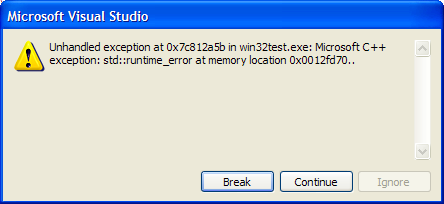
\includegraphics[height=3cm]{fig/exception2.png} 
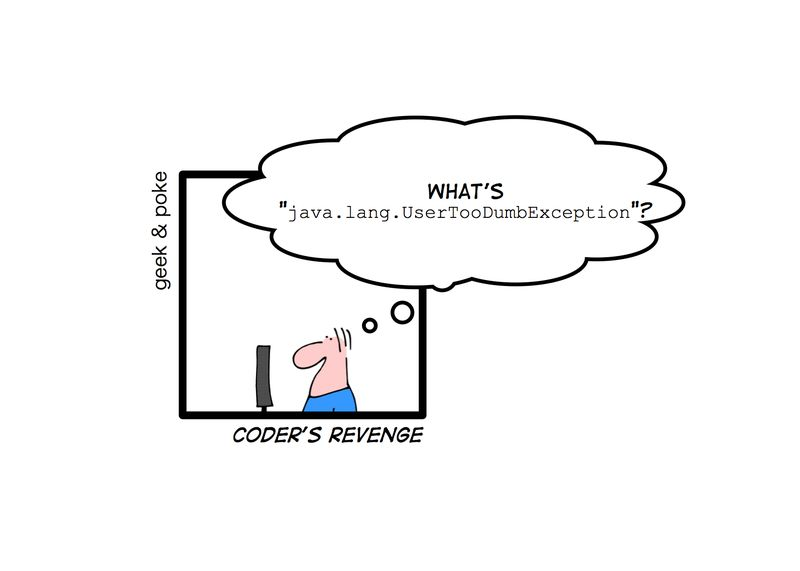
\includegraphics[height=3cm]{fig/usertoodumb.jpg}
\end{center}
\end{frame}

\begin{frame}{Que peut-on faire ?}
\begin{itemize}
\item Erreurs de compilation : facile !
\item Des tests !
\begin{itemize}
\item Voir le cours de MEDEV pour les tests unitaires, tests d'intégration, plans de tests
\item Mais aussi : la preuve de programme ou de propriétés, etc. 
\end{itemize}
\item Vérifier que tout se passe bien pendant l'exécution du programme
\begin{itemize}
\item Vérifier que les actions de l'utilisateur sont valides
\item Vérifier que certaines valeurs de variables sont appropriées (assertions)
\item Ne pas juste planter un programme quand quelque chose ne va pas
\end{itemize}
\item Pour autant, on ne va pas y passer notre vie...
\end{itemize}
\end{frame}

\subsection{Les assertions}

\begin{frame}[fragile]\frametitle{Les assertions : arrêter un programme à temps}
\begin{itemize}
\item \structure{pré-conditions} : on sait que certaines fonctions s'exécutent dans certaines conditions 
\item Sans aller jusqu'à la \href{http://fr.wikipedia.org/wiki/Programmation_par_contrat}{programmation par contrat}, on peut valider certaines pré-conditions importantes
\item C'est l'étape qui suit ... l'écriture des pré-conditions dans la documentation !
\item Mieux vaut les utiliser en mode debug que production
\end{itemize}
\begin{codeblock}{Exemple}
\begin{lstlisting}
#include <cassert>
using namespace std;

bool compte::debiter(float montant) {
    assert((montant >= 0));
    if (!ib && solde>=montant) {
        solde -= montant;
        return true;
    }
    return false;
}
\end{lstlisting}
\end{codeblock}
\end{frame}

\begin{frame}[fragile]\frametitle{Résultat}
\begin{itemize}
%\item Si l'assertion est vérifiée, rien ne se passe
\item Si l'assertion n'est pas vérifiée, message d'erreur et arrêt du programme
\begin{block}{Résultat avec un débit de -1000}
{\tiny 
\begin{verbatim}
Assertion failed: ((montant >= 0)), function debiter, file /Users/moreau/Documents/Enseignement/optionRV/CPLUS/code/compte.cxx, line 26.
Abort
\end{verbatim}}
\end{block}
\item Il vaut mieux utiliser des assertions claires...
\item \alert{Attention} : l'assertion est une technique de détection des erreurs de programmation et non pas de gestion des erreurs d'exécution !
\begin{itemize}
\item En clair, elles sont réservées au développeur 
\item Les assertions ne sont pas vérifiées dans un programme compilé en mode Release
\item Conséquence : éviter les expressions du type \verb|assert(index++ < MAXVAL)|
\item On peut les supprimer en compilant avec \verb|-DNDEBUG|
\end{itemize}
\end{itemize}
\end{frame}


\subsection{Utilisation des exceptions en C++}

\begin{frame}[fragile]
\frametitle{Exemple introductif}
\begin{itemize}
\item C++ ne nous facilite pas énormément la vie par défaut pour la gestion des erreurs 
\end{itemize}
\begin{codeblock}{Exemple}
\begin{lstlisting}
int division(int a, int b) {
    return a/b;
}

int main() {
    int tab[SZ];
    char * a = "lorsque l'enfant parait, son doux regard qui brille...";
    for (int i=0 ; i<=SZ+1 ; i++) {
        tab[i] = i*i;
    }
    
    for (int i=0 ; i<=SZ+1 ; i++) {
        std::cout << "tab[" << i << "] = " << tab[i] << std::endl;
    }
    
    std::cout << a << std::endl;
    
    std::cout << division(24,4) << std::endl;
    std::cout << division(24,0) << std::endl;
    
}
\end{lstlisting}
\end{codeblock}
\end{frame}

\begin{frame}[fragile]
\frametitle{Résultat}
\begin{block}{Exécution (pas forcément répétable)}
{\tiny 
\begin{verbatim}
tab[0] = 0
tab[1] = 1
tab[2] = 4
tab[3] = 9
tab[4] = 16
tab[5] = 25
tab[6] = 36
tab[7] = 49
tab[8] = 64
tab[9] = 81
tab[10] = 100
tab[11] = 121
lorsque l'enfant parait, son doux regard qui brille...
6
Floating exception
\end{verbatim}
}
\end{block}
\begin{itemize}
\item Les dépassements de tableau peuvent avoir une incidence ... ou pas
\item La division par zéro fait planter le programme
\end{itemize}
\end{frame}

\begin{frame}[fragile]
\frametitle{Quelques possibilités pour gérer les erreurs (1/2)}
\begin{itemize}
\item Renvoyer une valeur prédéfinie à la place du résultat
\begin{lstlisting}
#define ERROR_DIV_BY_0 -125

int division(int a, int b) {
    if (b !=0 ) {
        return a/b;
    }
    else {
        return ERROR_DIV_BY_0;
    }
}
\end{lstlisting}
\begin{itemize}
\item il faudrait être sûr que la valeur de \verb|ERROR_DIV_BY_0| n'est pas un résultat possible
\item l'utilisateur de la division va-t-il vraiment s'en soucier ?
\end{itemize}
\item Afficher un message d'erreur
\begin{lstlisting}
        std::cerr << "tentative de division par 0" << std::endl;
\end{lstlisting}
\begin{itemize}
\item message pour l'utilisateur final ? dans un programme avec GUI ?
\item Valeur de retour de la fonction dans ce cas ?
\end{itemize}
\end{itemize}
\end{frame}

\begin{frame}[fragile]
\frametitle{Quelques possibilités pour gérer les erreurs (2/2)}
\begin{itemize}
\item Gestion des erreurs "à la C" : retour de la fonction booléen et passage de la vraie valeur par adresse
\begin{lstlisting}
bool division_faconC(int a,int b,int &r) {
    if (b != 0) {
        r = a/b;
        return true;
    }
    else {
        return false;
    }
}
\end{lstlisting}
\begin{itemize}
\item Lourd mais efficace
\item Franchement pas intuitif
\end{itemize}
\end{itemize}
\end{frame}

\begin{frame}{Principe des exceptions}
\begin{itemize}
\item On va délimiter les zones \textit{à risque} d'un programme, c'est-à-dire les zones où il peut se produire quelque chose d'anormal
\item Si une erreur survient dans ces zones, on \struc{lève une exception} à l'aide d'un objet qui contient des informations sur l'erreur
\item Quelque part dans le code (à l'endroit où c'est le plus approprié), on gère l'erreur en \struc{attrapant l'exception} 
\item Si aucun code n'attrape l'exception, le programme s'arrête
\end{itemize}
\end{frame}

\begin{frame}[fragile]\frametitle{Les exceptions en C++}
\begin{itemize}
\item Les exceptions en C++ font appel à trois mots-clés
\begin{itemize}
\item \verb|try{ ... }| délimite le morceau de code susceptible de lever des exceptions
\item \verb|throw| \textit{expression} permet de lever une exception
\begin{itemize}
\item \verb|throw| doit de préférence se trouver dans un bloc \verb|try { ... }|
\end{itemize}
\item \verb|catch(...) { ... }| permet d'attraper une exception
\begin{itemize}
\item Les blocs \verb|catch(...) { ... }| suivent obligatoirement un bloc \verb|try { ... }|
\item On peut associer plusieurs \verb|catch| à un seul \verb|try|, il en faut au moins un par type d'\textit{expression} lancée par le \verb|throw|
\end{itemize}
\end{itemize}
\end{itemize}
\end{frame}

\begin{frame}[fragile]
\frametitle{Exemple : gestion de la division par zéro (1/2)}
\begin{enumerate}
\item Inclusion d'un bloc \verb|try|
\item Ajout d'un \verb|throw| pour lever une exception
\item Ajout d'un bloc \verb|catch|
\end{enumerate}
\begin{lstlisting}
int division(int a, int b) {
    try {
        if (b !=0 ) {
            return a/b;
        }
        else {
            throw std::string("Division par zero !");
        }
    }
    catch (std::string const& err_msg) {
        std::cerr << "Exception: " << err_msg << std::endl;
    }
}
\end{lstlisting}
\begin{itemize}
\item On est retourné au simple affichage du message d'erreur...
\begin{itemize}
\item Parce qu'on ne gère pas l'erreur à l'endroit approprié
\end{itemize}
\end{itemize}
\end{frame}

\begin{frame}[fragile]
\frametitle{Exemple : gestion de la division par zéro (2/2)}
\begin{itemize}
\item Nouvelle version 
\begin{itemize}
\item Plus de \verb|try| dans la fonction division mais dans son utilisation
\end{itemize}
\begin{lstlisting}
int division(int a, int b) {
        if (b !=0 ) {
            return a/b;
        }
        else {
            throw std::string("Division par zero !");
        }
}
\end{lstlisting}
\item Le code après le \verb|throw| n'est pas exécuté, donc pas de problème de valeur de retour
\item Utilisation
\begin{lstlisting}
    try {
        std::cout << division(24,4) << std::endl;
        std::cout << division(24,0) << std::endl;
    }
    catch(const std::string& err_msg) {
        std::cerr << "Exception : " << err_msg << std::endl;
    }
\end{lstlisting}
\end{itemize}
\end{frame}

\begin{frame}{Plus formellement...}
\begin{itemize}
	\item Une exception est un signal
	\begin{itemize}
		\item qui indique que quelque chose d'exceptionnel (par exemple une erreur) s'est produit
		\item qui interrompt le flot d'exécution normal du programme
	\end{itemize}
	\item lancer (\textbf{\texttt{throw}}) une exception revient à signaler quelque chose
	\item attraper (\textbf{\texttt{catch}}) une exception permet d'exécuter les actions nécessaires au traitement de la situation particulière
\end{itemize}
\end{frame} 


%%%%%%%%%%%%%%%%%%%%%%%%%%%%%%%%%%%%%%%%%%%%%%%%
\begin{frame}{Les exceptions : mécanisme}
\begin{itemize}
	\item lorsqu'une situation exceptionnelle est rencontrée une exception est lancée
	\item si cette exception n'est pas attrapée dans le bloc de code dans lequel elle se trouve, elle est propagée au bloc de code supérieur et ainsi de suite...
	\item même principe pour les fonctions/méthodes...
	\item si une exception n'est jamais attrapée :
	\begin{itemize}
		\item propagation jusqu'au main()
		\item affichage d'un message d'erreur
		\item arrêt de l'exécution du programme
	\end{itemize}
\end{itemize}
\end{frame} 

\begin{frame}{Pourquoi des objets Exception ?}
\begin{itemize}
	\item \alert{Transparent issu du cours de Java !}
	\item La représentation des objets sous forme d'objets permet de mieux structurer la description et le traitement des erreurs
\end{itemize}
{\small \begin{quote}
"Because all exceptions that are thrown within a Java program 
are first-class objects, grouping or categorization of exceptions 
is a natural outcome of the class hierarchy.  Java exceptions 
must be instances of Throwable or anyThrowable descendant. 
As for other Java classes, you can create subclasses of the 
Throwable class and subclasses of yoursubclasses. 
Each "leaf" class (a class with no subclasses) represents 
a specific type of exception and each "node" class (a class with 
one or more subclasses) represents a group of 
related exceptions. "
\end{quote}}
\end{frame} 

\begin{frame}[fragile]\frametitle{Les objets \texttt{exception}}
\begin{itemize}
\item En C++, on peut lancer des exceptions de n'importe quel type
\item Pour mieux comprendre ce qui s'est passé, il serait intéressant d'avoir
\begin{itemize}
\item une description de l'erreur
\item l'endroit où elle se situe (fichier, ligne, pile d'appels)
\item d'éventuelles informations complémentaires selon l'erreur
\end{itemize}
\item La bibliothèque standard de C++ fournit une classe \verb|exception|
\begin{itemize}
\item Utilisation avec \verb|#include <exception>|
\item Les méthodes sont virtuelles, polymorphisme plus que recommandé
\end{itemize}
\item Pourquoi construire des classes dérivées de \verb|exception| ?
\begin{itemize}
\item Gérer ses propres erreurs
\item Hiérarchiser les types d'erreurs
\item Profiter de cette hiérarchie dans les bloc \verb|catch|
\end{itemize}
\end{itemize}
\end{frame}

\begin{frame}[fragile]\frametitle{Quelques classes dérivées d'\texttt{exception} (1/2)}
Exceptions susceptibles d'être levées par la bibliothèque standard
\begin{tabular}{|l|l|}
\hline Classe & Description \\ 
\hline \verb|bad_alloc| & Problème d'allocation mémoire \\ 
\hline \verb|bad_cast| & Erreur lors d'un \verb|dynamic_cast| \\
\hline \verb|bad_exception| & Pas de \verb|catch| correspondant à une exception levée \\
\hline \verb|bad_typeid| & erreur à l'utilisation de \verb|typeid| \\
\hline \verb|ios_base::failure| & problème avec un flot de données \\
\hline
\end{tabular} 
\end{frame}

\begin{frame}[fragile]\frametitle{Quelques classes dérivées d'\texttt{exception} (2/2)}
Quelques types d'exceptions pré-définies (dans \verb|stdexcept|) à réutiliser
\begin{tabular}{|l|l|}
\hline Classe & Description \\ 
\hline \verb|domain_error| & Erreur de domaine (maths) \\
\hline \verb|invalid_argument| & argument invalide (en valeur) passé à une fonction \\
\hline \verb|length_error| & taille invalide \\
\hline \verb|out_of_range| & erreur d'indice de tableau \\
\hline \verb|logic_error| & erreur logique (algo) \\
\hline
\end{tabular}
\begin{itemize}
\item Par exemple, dans l'exemple de la division, on aurait pu lever une \verb|domain_error|
\item \verb|out_of_range| pourrait être utilisé par \verb|vector<?>| pour signaler un indice hors limite
\begin{itemize}
\item En réalité, on aura plutôt un \verb|vector::_M_range_check|
\end{itemize} 
\end{itemize} 
\end{frame}